% Source: printed p. 471; PDF p. 480
\begin{figure}[p]
\centering
\begin{tikzpicture}[font=\small,scale=.85]
\draw[red](2.15,3.2)ellipse(3.5 and 2.5);
\draw(0,3.25)--(0,4.55)--(1.35,3.9)--cycle;\node at(.45,3.9){$f_1$};
\foreach\y/\l in {4.35/A,3.9/B,3.45/C}{\draw(-.5,\y)--(0,\y);\node[above]at(-.35,\y){$\l$};}
\draw(0,1.4)--(0,2.7)--(1.35,2.05)--cycle;\node at(.45,2.05){$f_2$};\draw(-.5,2.05)--(0,2.05);\node[above]at(-.35,2.05){$D$};
\draw(2.9,2.25)--(2.9,3.65)--(4.25,2.95)--cycle;\node at(3.35,2.95){$g$};
\draw(1.35,3.9)--(1.8,3.9)node[above]{$S$}..controls(2.6,3.9)and(2.05,3.15)..(2.9,3.15);
\draw(1.35,2.05)--(1.8,2.05)node[above]{$T$}..controls(2.6,2.05)and(2.05,2.75)..(2.9,2.75);
\draw(4.25,2.95)--(4.7,2.95);\node[above]at(4.55,2.95){$X$};
\draw[red](4.9,4.25)--(8.3,.65);\draw[red](-.15,1.1)--(4.2,-1.7);
\node[align=center,text width=3.8cm,font=\footnotesize,fill=white,inner sep=2pt]at(1.6,.2){các cấu xạ ở trên\\hợp thành để cho ra};
\draw[red](6.2,-.7)ellipse(2.6 and 1.75);
\draw(5.1,-1.7)--(5.1,.3)--(7.6,-.7)--cycle;\node[font=\scriptsize]at(5.95,-.7){$g\circ(f_1,f_2)$};
\foreach\y/\l in {.2/A,-.4/B,-1/C,-1.6/D}{\draw(4.6,\y)--(5.1,\y);\node[above,font=\scriptsize]at(4.8,\y){$\l$};}
\draw(7.6,-.7)--(8.03,-.7);\node[above]at(7.85,-.7){$X$};
\end{tikzpicture}
\setcounter{figure}{3}
\caption{Phép hợp thành các cấu xạ $f_1$ và $f_2$ với $g$.}
\label{fig:ctseven-operad-composition}
\end{figure}
\clearpage

% Source: printed p. 472; PDF p. 481
\begin{figure}[p]
\centering
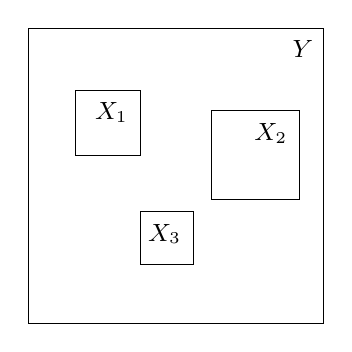
\begin{tikzpicture}[font=\small,scale=.75]
\draw(0,0)rectangle(5,5);\node at(4.65,4.65){$Y$};
\draw(.8,2.85)rectangle(1.9,3.95);\node[anchor=north east]at(1.85,3.9){$X_1$};
\draw(3.1,2.1)rectangle(4.6,3.6);\node[anchor=north east]at(4.55,3.55){$X_2$};
\draw(1.9,1)rectangle(2.8,1.9);\node[anchor=north east]at(2.75,1.85){$X_3$};
\end{tikzpicture}
\setcounter{figure}{4}
\caption{Một cấu xạ $(X_1,X_2,X_3)\to Y$ trong một operad chỉ có một đối tượng, $\square$.}
\label{fig:ctseven-little-squares}
\end{figure}

\begin{figure}[p]
\centering
\begin{tikzpicture}[font=\scriptsize,scale=.85]
\draw(0,1)rectangle(1,2);\node[anchor=south east]at(.97,2.08){$X_1$};\draw(.36,1.57)rectangle(.56,1.77);\draw(.36,1.21)rectangle(.56,1.41);
\draw(1.65,1)rectangle(2.65,2);\node[anchor=south east]at(2.62,2.08){$X_2$};\draw(1.75,1.62)rectangle(1.99,1.86);\draw(2.27,1.37)rectangle(2.44,1.54);\draw(2.27,1.1)rectangle(2.44,1.27);
\draw(3.3,1)rectangle(4.3,2);\node[anchor=south east]at(4.27,2.08){$X_3$};\draw(3.57,1.66)rectangle(3.75,1.84);
\node at(5.05,1.5){\scalebox{1.8}{$\circ$}};
\begin{scope}[shift={(5.8,0)}]
\draw(0,0)rectangle(4,4);\node at(3.7,3.7){$Y$};
\draw(.65,2.28)rectangle(1.5,3.13);\node[anchor=north east]at(1.48,3.1){$X_1$};
\draw(2.5,1.68)rectangle(3.68,2.86);\node[anchor=north east]at(3.66,2.84){$X_2$};
\draw(1.55,.8)rectangle(2.25,1.5);\node[anchor=north east]at(2.23,1.48){$X_3$};
\end{scope}
\node at(3,-2.3){\scalebox{1.8}{$=$}};
\begin{scope}[shift={(3.8,-4.4)}]
\draw(0,0)rectangle(4,4);\node at(3.7,3.7){$Y$};
\draw(.956,2.765)rectangle(1.126,2.935);\draw(.956,2.459)rectangle(1.126,2.629);
\draw(2.618,2.412)rectangle(2.901,2.695);\draw(3.232,2.117)rectangle(3.433,2.318);\draw(3.232,1.798)rectangle(3.433,1.999);
\draw(1.739,1.262)rectangle(1.865,1.388);
\end{scope}
\end{tikzpicture}
\setcounter{figure}{5}
\caption{Một cấu xạ $(X_1,X_2,X_3)\to Y$ và các cấu xạ $(W_{1,1},W_{1,2})\to X_1$, $(W_{2,1},W_{2,2},W_{2,3})\to X_2$ và $(W_{3,1})\to X_3$, mỗi cấu xạ là một cách đặt các hình vuông vào trong một hình vuông. Công thức hợp thành được cho bằng cách co giãn và đặt các hình vuông để được $(W_{1,1},W_{1,2},W_{2,1},W_{2,2},W_{2,3},W_{3,1})\to Y$.}
\label{fig:ctseven-square-substitution}
\end{figure}
\clearpage

% Source: printed p. 473; PDF p. 482
\begin{figure}[p]
\centering
\definecolor{ctsevenmaterialback}{RGB}{211,222,235}
\definecolor{ctsevenmaterialred}{RGB}{200,77,87}
\definecolor{ctsevenmaterialblue}{RGB}{95,147,208}
\definecolor{ctsevenmaterialpurple}{RGB}{214,204,231}
\definecolor{ctsevenmaterialgreen}{RGB}{227,239,199}
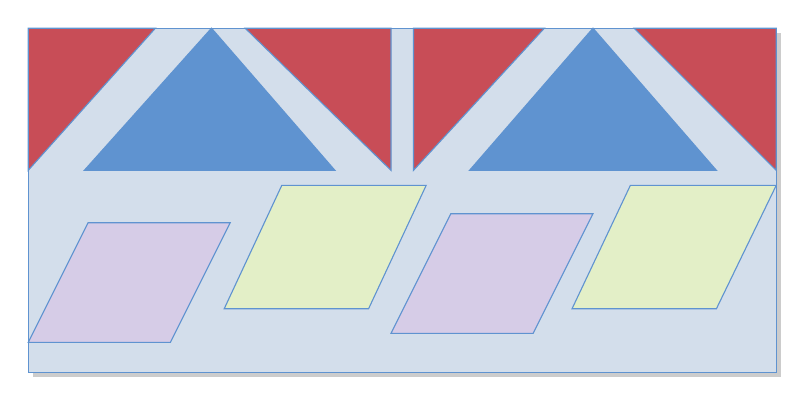
\begin{tikzpicture}[scale=.95]
\fill[gray!40](.06,-.06)rectangle(10.06,4.54);
\filldraw[fill=ctsevenmaterialback,draw=ctsevenmaterialblue](0,0)rectangle(10,4.6);
\foreach\a/\b/\c in {0/1.7/0,2.9/4.85/4.85,5.15/6.9/5.15,8.1/10/10}{\filldraw[fill=ctsevenmaterialred,draw=ctsevenmaterialblue](\a,4.6)--(\b,4.6)--(\c,2.7)--cycle;}
\filldraw[fill=ctsevenmaterialblue,draw=ctsevenmaterialblue](.75,2.7)--(4.1,2.7)--(2.45,4.6)--cycle;
\filldraw[fill=ctsevenmaterialblue,draw=ctsevenmaterialblue](5.9,2.7)--(9.2,2.7)--(7.55,4.6)--cycle;
\filldraw[fill=ctsevenmaterialpurple,draw=ctsevenmaterialblue](0,.4)--(1.9,.4)--(2.7,2)--(.8,2)--cycle;
\filldraw[fill=ctsevenmaterialpurple,draw=ctsevenmaterialblue](4.85,.52)--(6.75,.52)--(7.55,2.12)--(5.65,2.12)--cycle;
\filldraw[fill=ctsevenmaterialgreen,draw=ctsevenmaterialblue](2.62,.85)--(4.55,.85)--(5.32,2.5)--(3.39,2.5)--cycle;
\filldraw[fill=ctsevenmaterialgreen,draw=ctsevenmaterialblue](7.27,.85)--(9.2,.85)--(10,2.5)--(8.05,2.5)--cycle;
\end{tikzpicture}
\setcounter{figure}{6}
\caption{Một cấu xạ biểu thị cách xây dựng một vật liệu từ các vật liệu nhỏ hơn.}
\label{fig:ctseven-material-construction}
\end{figure}
\clearpage

% Source: printed p. 474; PDF p. 483
\begin{figure}[p]
\centering
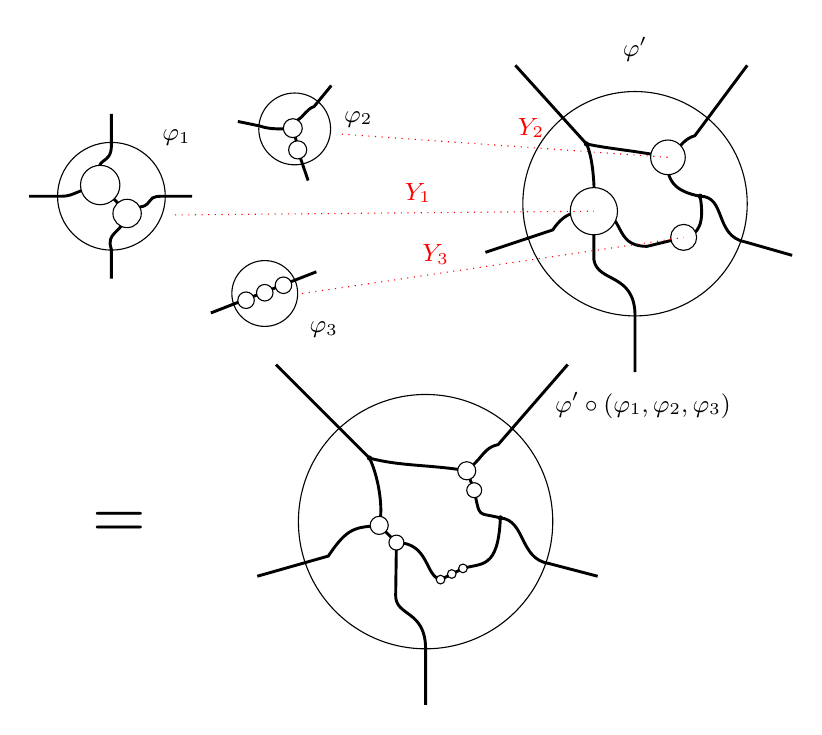
\begin{tikzpicture}[font=\small,scale=.95,wire/.style={line width=1.05pt},hole/.style={draw,circle,fill=white,inner sep=0pt}]
% phi_1: four outer ports, two inner circles, one internal wire.
\begin{scope}[shift={(0,3)}]
\draw(0,0)circle(.72);\node[above right]at(.55,.55){$\varphi_1$};
\draw[wire](-1.1,0)--(-.66,0)..controls(-.5,0)and(-.43,.1)..(-.25,.1);
\draw[wire](0,1.1)--(0,.68)..controls(0,.4)and(-.23,.55)..(-.15,.25);
\draw[wire](-.03,.03)--(.17,-.18);
\draw[wire](.29,-.15)..controls(.6,-.15)and(.42,0)..(.67,0)--(1.08,0);
\draw[wire](.17,-.31)..controls(.13,-.49)and(-.08,-.49)..(0,-.71)--(0,-1.1);
\node[hole,minimum size=5mm]at(-.15,.15){};\node[hole,minimum size=3.6mm]at(.21,-.23){};
\end{scope}
% phi_2: three outer ports, two inner circles.
\begin{scope}[shift={(2.45,3.9)}]
\draw(0,0)circle(.48);\node[right]at(.53,.13){$\varphi_2$};
\draw[wire](-.76,.1)--(-.47,.04)..controls(-.35,0)and(-.26,0)..(-.15,0);
\draw[wire](.49,.58)--(.26,.3)..controls(.15,.26)and(.12,.16)..(.03,.11);
\draw[wire](0,-.08)--(.035,-.21);\draw[wire](.06,-.34)--(.18,-.69);
\node[hole,minimum size=2.4mm]at(-.025,.01){};\node[hole,minimum size=2.3mm]at(.04,-.28){};
\end{scope}
% phi_3: three internal circles in a chain between two outer ports.
\begin{scope}[shift={(2.05,1.7)}]
\draw(0,0)circle(.44);\node[below right]at(.47,-.25){$\varphi_3$};
\draw[wire](-.72,-.26)--(.69,.29);
\node[hole,minimum size=2.1mm]at(-.25,-.09){};\node[hole,minimum size=2.1mm]at(0,.01){};\node[hole,minimum size=2.1mm]at(.25,.11){};
\end{scope}
% Outer morphism phi': five outer ports, three holes, two genuine wire junctions.
\begin{scope}[shift={(7,2.9)}]
\draw(0,0)circle(1.5);\node[above]at(0,1.77){$\varphi'$};
\draw[wire](-1.6,1.85)--(-.65,.8)..controls(-.4,.74)and(.08,.7)..(.44,.62);
\draw[wire](-.65,.8)..controls(-.57,.65)and(-.53,.24)..(-.55,-.1);
\draw[wire](1.5,1.85)--(.8,.91)..controls(.63,.86)and(.6,.73)..(.44,.62);
\draw[wire](-2,-.65)--(-1.1,-.35)..controls(-.92,-.08)and(-.74,-.1)..(-.55,-.1);
\draw[wire](-.55,-.1)..controls(-.1,-.1)and(-.32,-.57)..(.16,-.57)--(.65,-.45);
\draw[wire](-.55,-.1)--(-.55,-.75)..controls(-.5,-1.06)and(0,-.92)..(0,-1.5)--(0,-2.25);
\draw[wire](.44,.62)..controls(.4,.3)and(.55,.16)..(.87,.1);
\draw[wire](.87,.1)..controls(.93,-.25)and(.86,-.42)..(.65,-.45);
\draw[wire](.87,.1)..controls(1.22,.1)and(1.06,-.43)..(1.47,-.51)--(2.1,-.69);
\fill(-.65,.8)circle(.035);\fill(.87,.1)circle(.035);
\node[hole,minimum size=6mm](y1)at(-.55,-.1){};\node[hole,minimum size=4.4mm](y2)at(.44,.62){};\node[hole,minimum size=3.3mm](y3)at(.65,-.45){};
\end{scope}
\draw[red,dotted](.85,2.75)--(6.45,2.8)node[pos=.58,above]{$Y_1$};
\draw[red,dotted](3.08,3.83)--(7.44,3.52)node[pos=.58,above]{$Y_2$};
\draw[red,dotted](2.55,1.7)--(7.65,2.45)node[pos=.35,above]{$Y_3$};
\node at(.1,-1.4){\scalebox{2.7}{$=$}};
% Composite: the same five external ports; all seven inner circles survive substitution.
\begin{scope}[shift={(4.2,-1.35)}]
\draw(0,0)circle(1.7);\node[above right]at(1.6,1.25){$\varphi'\circ(\varphi_1,\varphi_2,\varphi_3)$};
\draw[wire](-2,2.1)--(-.75,.85)..controls(-.35,.74)and(.1,.76)..(.55,.68);
\draw[wire](-.75,.85)..controls(-.63,.6)and(-.56,.18)..(-.62,-.05);
\draw[wire](1.9,2.1)--(.97,1.03)..controls(.78,.99)and(.78,.87)..(.55,.68);
\draw[wire](-2.25,-.73)--(-1.3,-.46)..controls(-1.04,-.07)and(-.94,-.08)..(-.62,-.05);
\draw[wire](-.62,-.05)--(-.39,-.28);
\draw[wire](-.39,-.28)..controls(.05,-.28)and(-.01,-.73)..(.2,-.775)--(.5,-.625)..controls(.75,-.55)and(.97,-.64)..(1,.05);
\draw[wire](-.39,-.28)--(-.4,-.99)..controls(-.4,-1.27)and(0,-1.18)..(0,-1.7)--(0,-2.45);
\draw[wire](.55,.68)--(.65,.42)..controls(.73,.03)and(.69,.13)..(1,.05);
\draw[wire](1,.05)..controls(1.34,.02)and(1.25,-.5)..(1.65,-.56)--(2.3,-.73);
\fill(-.75,.85)circle(.035);\fill(1,.05)circle(.035);
\node[hole,minimum size=2.3mm]at(-.62,-.05){};\node[hole,minimum size=1.9mm]at(-.39,-.28){};
\node[hole,minimum size=2.3mm]at(.55,.68){};\node[hole,minimum size=1.9mm]at(.65,.42){};
\foreach\x/\y in {.2/-.775,.35/-.70,.5/-.625}{\node[hole,minimum size=1.1mm]at(\x,\y){};}
\end{scope}
\end{tikzpicture}
\setcounter{figure}{7}
\caption{Các cấu xạ trong một operad sơ đồ nối dây $\mathcal W$. Phép hợp thành các sơ đồ nối dây được cho bằng phép thế.}
\label{fig:ctseven-wiring-substitution}
\end{figure}
\clearpage
